\ejercicio
Determinar si $A \subseteq B$ en cada uno de los siguientes casos:

\separadorCorto

Inclusión :
$
	\begin{cases}
		\text{Definición}      & A \subseteq B \text{ si } \paratodo x, x \en A \entonces x \en B   \\
		\text{Contrarecíproco} & A \nsubseteq B \text{ si } \existe x, x \en A \entonces x \notin B
	\end{cases}
$
\begin{enumerate}[label=(\roman*)]
	\item $\begin{cases}
			      A = \set{1, 2, 3} \\
			      B = \set{5,4,3,2,1}
		      \end{cases}
		      \flecha{respueta} \quad
		      A \stacktext{\Tilde}{\subseteq} B$
	\item $\begin{cases}
			      A = \set{1, 2, 3} \\
			      B = \set{1,2,\set{3},-3}
		      \end{cases}
		      \flecha{respueta} \quad
		      A \nsubseteq B \flecha{dado}[que] \set{3} \notin B$
	\item
	      \def\tresiiiUno{
		      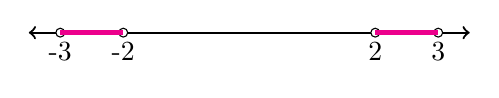
\begin{tikzpicture}[scale=0.8, baseline=0]
			      % Number line
			      \draw[thick, <->,] (-3.5,0) -- (3.5,0);
			      % Interval
			      \draw[fill=white] (2,0) circle (2pt);
			      \draw[fill=white] (3,0) circle (2pt);
			      \draw[fill=white] (-2,0) circle (2pt);
			      \draw[fill=white] (-3,0) circle (2pt);
			      \draw[-, magenta, ultra thick] (2,0) -- (3,0);
			      \draw[-, magenta, ultra thick] (-2,0) -- (-3,0);
			      \node at (2,-0.3) {2};
			      \node at (3,-0.3) {3};
			      \node at (-2,-0.3) {-2};
			      \node at (-3,-0.3) {-3};
		      \end{tikzpicture}
	      }

	      \def\tresiiiDos{
		      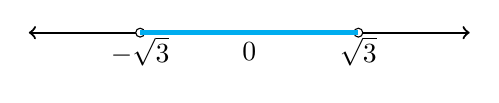
\begin{tikzpicture}[scale=0.8, baseline=0]
			      % Number line
			      \draw[thick, <->,] (-3.5,0) -- (3.5,0);
			      % Interval
			      \draw[fill=white] (1.732,0) circle (2pt);
			      \draw[fill=white] (-1.732,0) circle (2pt);
			      \draw[-, cyan, ultra thick] (1.732,0) -- (-1.732,0);
			      \node at (1.732,-0.3) {$\sqrt{3}$};
			      \node at (-1.732,-0.3) {$-\sqrt{3}$};
			      \node at (0,-0.3) {0};
		      \end{tikzpicture}
	      }
	      $
		      \llaves{ll}{
			      A = \set{x \en \reales \talque 2<|x|<3} & \tresiiiUno \\
			      B = \set{x \en \reales \talque x^2 < 3 } & \tresiiiDos
		      }\\
		      \flecha{respueta} A \nsubseteq B \flecha{dado}[que] 2.5 \en A \text{ y } 2.5 \not\en B
	      $
	\item
	      $
		      \begin{cases}
			      A = \set{\vacio} \\
			      B = \vacio
		      \end{cases}\\
		      \flecha{respueta}
		      A \nsubseteq B \flecha{dado}[que] \text{$B$ no tiene ningún elemento, sin embargo $A$ tiene un elemento: $\vacio$.}
	      $
\end{enumerate}
